\clearpage
\hypertarget{conBran vis}{}
\subsection{Branching with statement nodes}
\visHeader

\begin{itemize}

\item[$\blacktriangleright$] Currently, there isn't a method to help us initialize \texttt{box} from the state of no partitions. Create one by editing
your metamodel (the \texttt{LearningBoxLanguage} diagram) and invoking the \texttt{Operations} dialogue by first selecting \texttt{Box}, then pressing
\texttt{F10}.\footnote{To review creating new operations, review Section 2.6 of Part II}

\item[$\blacktriangleright$] Name the new method \texttt{initializeBox} and, recalling the one rule of conditional branching, set its return type to
\texttt{EBoolean}.

\item[$\blacktriangleright$] Save and close the dialogue, then re-open the \texttt{grow} SDM and \emph{Quick Create} a new activity node from
\texttt{addNewPartition}.

\item[$\blacktriangleright$] This will be the node we'll use to access our helper method. Unfortunately, the default is the wrong type of node.
Double click the element to invoke its properties editor and switch the \texttt{Type} to a \texttt{StatementNode}. Name it \texttt{initialize}
(Fig.~\ref{fig:newStatementNode}).

\item[$\blacktriangleright$] Before closing the dialogue, switch to the \texttt{Statement} tab, and invoke a \texttt{MethodCallExpression} to your newest
method (Fig.~\ref{fig:statementMCE}). We want to access the \texttt{Box} object (\texttt{this}) and its \texttt{initalizeBox} method. It doesn't require any
parameters, so leave the values field empty. 

\begin{figure}[htbp]
   \centering
      \subfloat[Create a new \emph{StatementNode}]{
        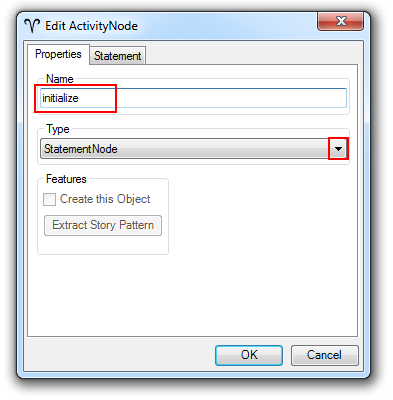
\includegraphics[width=0.5\textwidth]{ea_newStatementNode}
        \label{fig:newStatementNode}
      }
      \subfloat[Edit the \texttt{MethodCallExpression} ]{
        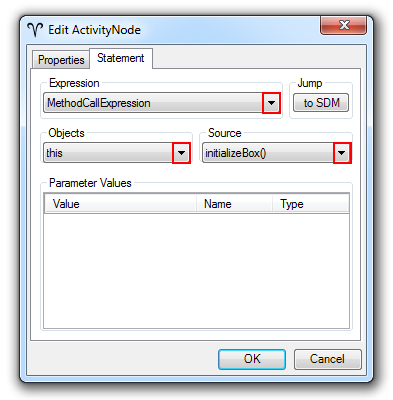
\includegraphics[width=0.5\textwidth]{ea_statementMCExpression}
        \label{fig:statementMCE}
      }
      \caption{}
\end{figure}
\FloatBarrier

\clearpage

\item[$\blacktriangleright$] Now we need to update the edge guards stemming from \texttt{add\-New\-Part\-ition\-In\-Box}. Given that we only want to call
\texttt{initializeBox} if \texttt{box} isn't able to execute the NAC, change the edge leading to your statement node to \texttt{Failure}. Similarly, update the
edge returning \texttt{true} to \texttt{Success}.

\item[$\blacktriangleright$] Finally, attach two stopnodes -- \texttt{true} and \texttt{false} -- along with their appropriate edge guards from
\texttt{initialize}. These indicate that if the method execution worked, the box could be initialized. If it failed however, \texttt{box} was
in an invalid state (by, i.e., having only one card) and returns \texttt{false}. Overall, the new additions to \texttt{box.grow()} should resemble Fig.~\ref{fig:newGrowControl}.

\vspace{0.5cm}

\begin{figure}[htp]
\begin{center}
  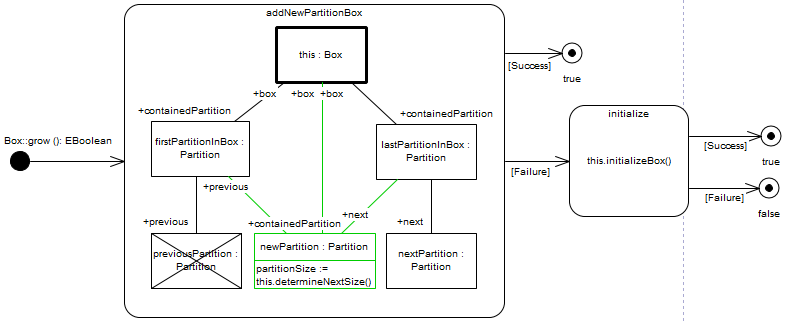
\includegraphics[width=\textwidth]{ea_growAdditions}
  \caption{Extending \texttt{grow} with a \emph{MethodCallExpression}}
  \label{fig:newGrowControl}
\end{center}
\end{figure}

\item[$\blacktriangleright$] To review our work up to this point, we have declared the \texttt{initializeBox} signature and invoked it from a node. We have yet
to actually specify the method however. You'll notice in (Fig.~\ref{fig:newStatementNode}) that the \texttt{Extract Story Pattern} option is invalid. This
makes sense -- you don't define a pattern in a statement node. Instead, double-click the anchor to return to the main diagram and create a new SDM
for \texttt{initializeBox}.

\item[$\blacktriangleright$] Create a normal activity node named \texttt{buildPartitions}. Within it, have a bound \texttt{Box} linked to a
\texttt{onePartition} NAC, and two other `green' (create) object variables, \texttt{firstPartition} and \texttt{lastPartition} with their links satisfied.

\item[$\blacktriangleright$] Finally, attach a true and false \texttt{StopNode} (with edge guards) to the node. The completed pattern should come to resemble
Fig.~\ref{fig:buildPartitions}.

\newpage
 
\begin{figure}[htp]
\begin{center}
  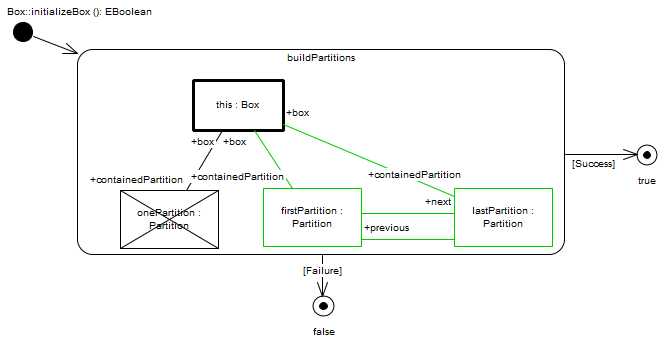
\includegraphics[width=\textwidth]{eclipse_buildPartitions}
  \caption{Compelted NAC to check for \emph{one} partition}
  \label{fig:buildPartitions}
\end{center}
\end{figure}
 
\item[$\blacktriangleright$] In summary, the NAC here can only fulfilled if the box has no partitions, i.e., is in a pristine state and able to be initialized.
In other words, if \texttt{grow} is used for an empty box, it initializes the box for the first time and grows it after that, ensuring that the box is always in
a valid state.
 
\item[$\blacktriangleright$] You're finished! Save, validate, and build your metamodel, then check out how this is done in the textual syntax in
Fig.~\ref{fig:updateGrow} and Fig.~\ref{fig:pattBuildParts}.

\jumpSingle{initialize notes}

\end{itemize}
